\documentclass{standalone}
\usepackage{tikz}
\usetikzlibrary{patterns, positioning}
\usepackage[sfdefault]{ClearSans} %% option 'sfdefault' activates Clear Sans as the default text font
\usepackage[T1]{fontenc}

\begin{document}
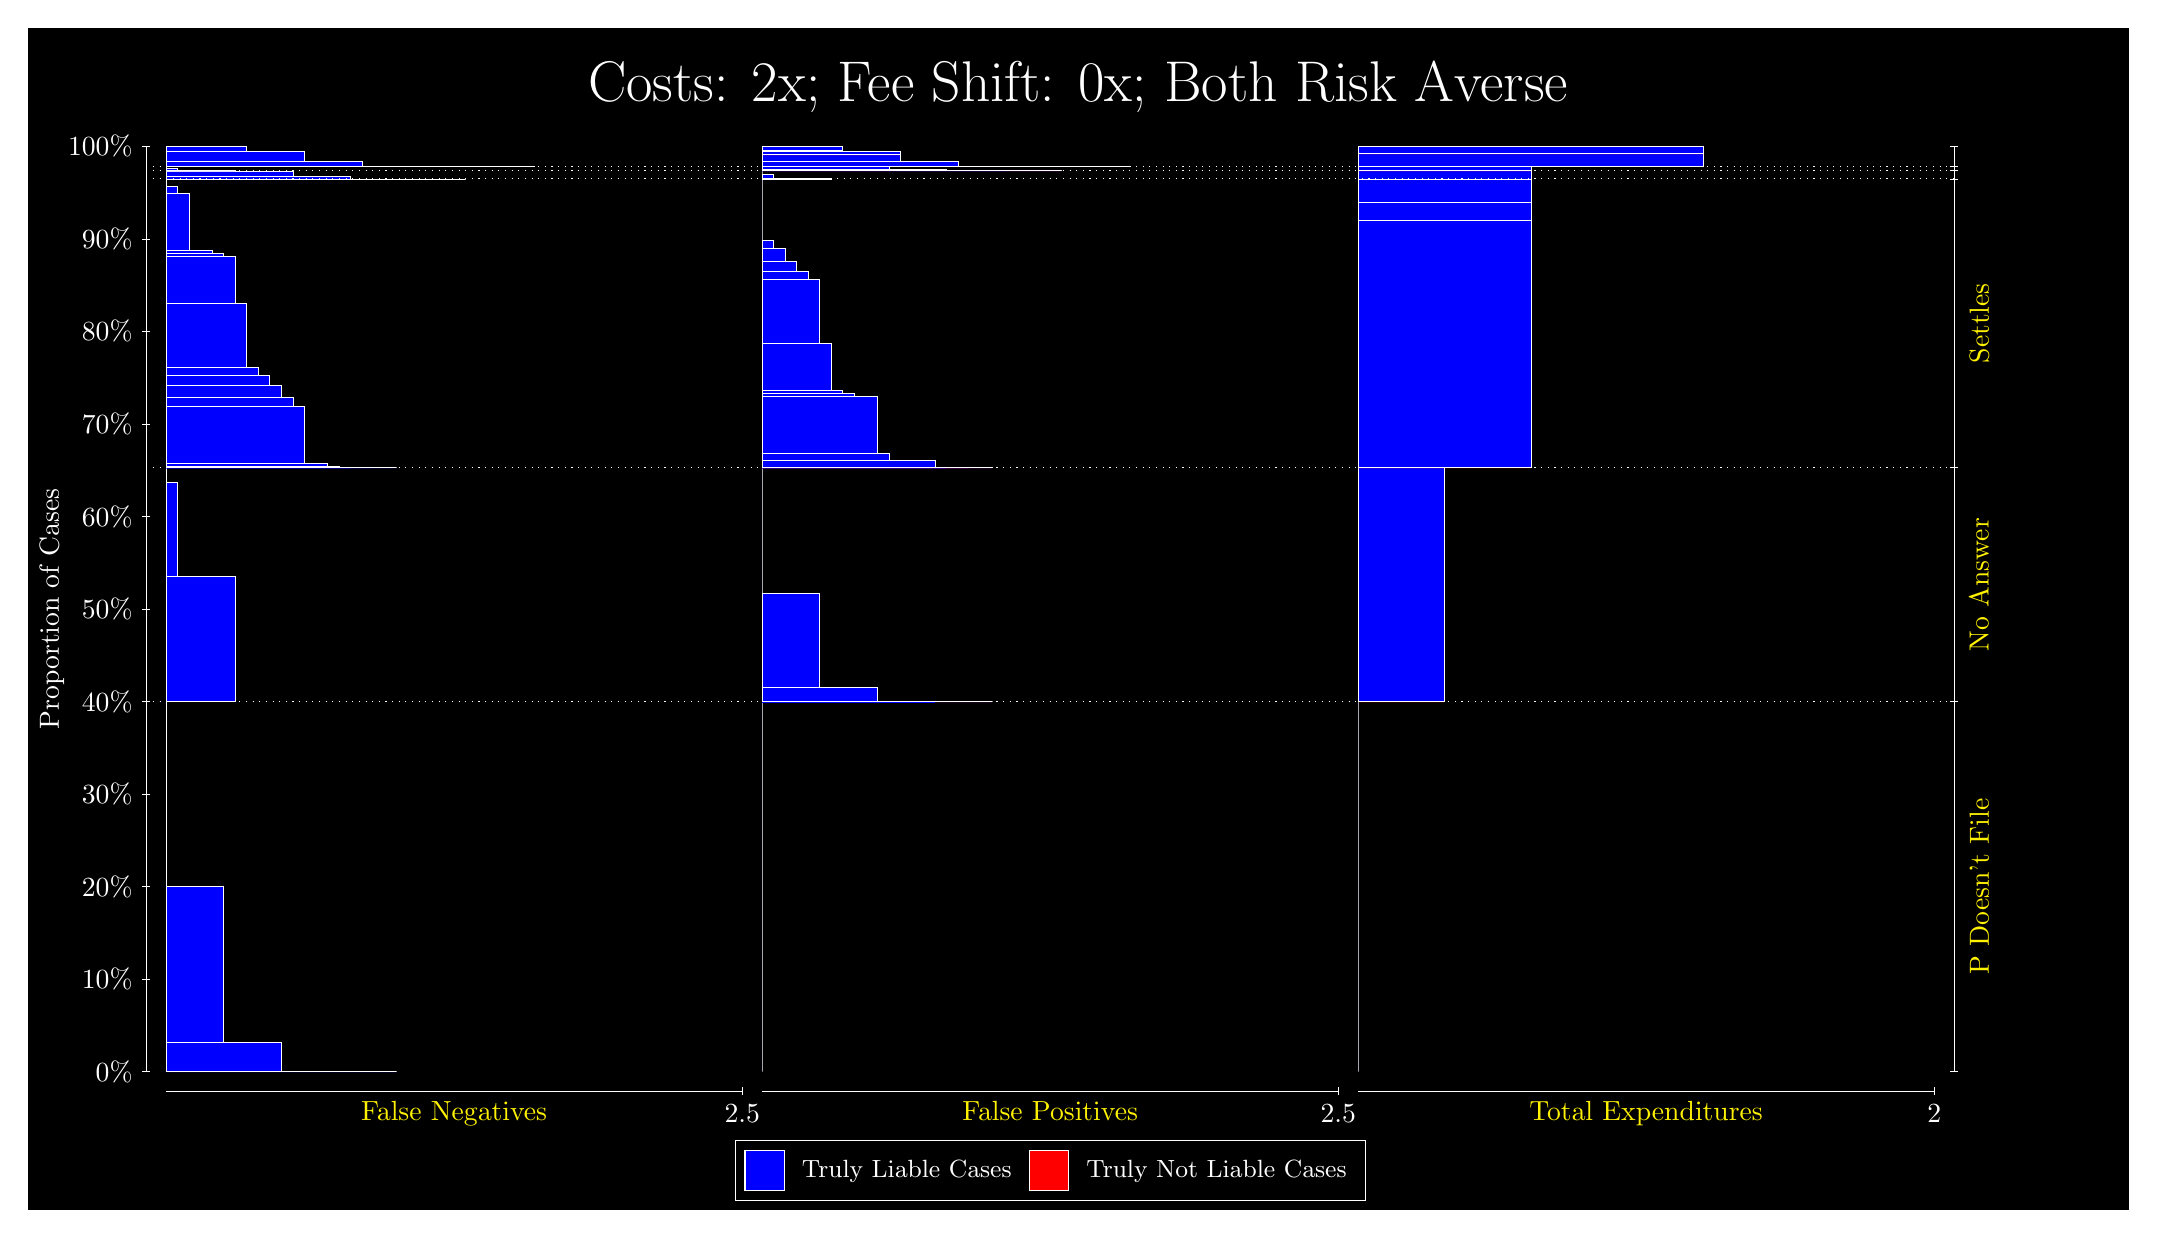
\begin{tikzpicture}
\draw[fill=black] (0,0) rectangle (26.667,15);
\draw[text=white] (0,13.5) rectangle (26.667,15) node[midway] {\huge Costs: 2x; Fee Shift: 0x; Both Risk Averse};
\draw[white, very thin] (1.5,1.75) -- (1.5,13.5);
\node[rotate=90, text=white, anchor=center] at (0.3, 7.625) {Proportion of Cases};
\draw[white, very thin] (1.45,1.75) -- (1.55,1.75);
\node[text=white, anchor=east] at (1.45, 1.75) {0\%};
\draw[white, very thin] (1.45,2.925) -- (1.55,2.925);
\node[text=white, anchor=east] at (1.45, 2.925) {10\%};
\draw[white, very thin] (1.45,4.1) -- (1.55,4.1);
\node[text=white, anchor=east] at (1.45, 4.1) {20\%};
\draw[white, very thin] (1.45,5.275) -- (1.55,5.275);
\node[text=white, anchor=east] at (1.45, 5.275) {30\%};
\draw[white, very thin] (1.45,6.45) -- (1.55,6.45);
\node[text=white, anchor=east] at (1.45, 6.45) {40\%};
\draw[white, very thin] (1.45,7.625) -- (1.55,7.625);
\node[text=white, anchor=east] at (1.45, 7.625) {50\%};
\draw[white, very thin] (1.45,8.8) -- (1.55,8.8);
\node[text=white, anchor=east] at (1.45, 8.8) {60\%};
\draw[white, very thin] (1.45,9.975) -- (1.55,9.975);
\node[text=white, anchor=east] at (1.45, 9.975) {70\%};
\draw[white, very thin] (1.45,11.15) -- (1.55,11.15);
\node[text=white, anchor=east] at (1.45, 11.15) {80\%};
\draw[white, very thin] (1.45,12.325) -- (1.55,12.325);
\node[text=white, anchor=east] at (1.45, 12.325) {90\%};
\draw[white, very thin] (1.45,13.5) -- (1.55,13.5);
\node[text=white, anchor=east] at (1.45, 13.5) {100\%};

\draw[white, very thin] (24.457,1.75) -- (24.457,13.5);
\draw[white, very thin] (24.407,1.75) -- (24.507,1.75);
\node[anchor=west] at (24.407, 1.75) {};
\draw[white, very thin] (24.407,6.4489) -- (24.507,6.4489);
\node[anchor=west] at (24.407, 6.4489) {};
\draw[white, very thin] (24.407,9.4191) -- (24.507,9.4191);
\node[anchor=west] at (24.407, 9.4191) {};
\draw[white, very thin] (24.407,13.087) -- (24.507,13.087);
\node[anchor=west] at (24.407, 13.087) {};
\draw[white, very thin] (24.407,13.19) -- (24.507,13.19);
\node[anchor=west] at (24.407, 13.19) {};
\draw[white, very thin] (24.407,13.245) -- (24.507,13.245);
\node[anchor=west] at (24.407, 13.245) {};
\draw[white, very thin] (24.407,13.5) -- (24.507,13.5);
\node[anchor=west] at (24.407, 13.5) {};

\draw[white, very thin, fill=blue] (1.75,1.75) rectangle (4.6775,1.75);
\draw[white, very thin, fill=blue] (1.75,1.75) rectangle (3.9457,1.7532);
\draw[white, very thin, fill=blue] (1.75,1.7532) rectangle (3.2138,2.126);
\draw[white, very thin, fill=blue] (1.75,2.126) rectangle (2.4819,4.1027);
\draw[white, very thin, fill=red] (1.75,4.1027) rectangle (1.75,4.1027);
\draw[white, very thin, fill=blue] (1.75,4.1027) rectangle (1.75,6.4489);
\draw[white, very thin, fill=blue] (1.75,6.4489) rectangle (2.6283,8.0449);
\draw[white, very thin, fill=blue] (1.75,8.0449) rectangle (1.8964,9.2363);
\draw[white, very thin, fill=red] (1.75,9.2363) rectangle (1.75,9.2363);
\draw[white, very thin, fill=blue] (1.75,9.2363) rectangle (1.75,9.4191);
\draw[white, very thin, fill=blue] (1.75,9.4191) rectangle (4.6775,9.4191);
\draw[white, very thin, fill=blue] (1.75,9.4191) rectangle (4.3848,9.4191);
\draw[white, very thin, fill=blue] (1.75,9.4191) rectangle (4.092,9.4193);
\draw[white, very thin, fill=blue] (1.75,9.4193) rectangle (3.9457,9.442);
\draw[white, very thin, fill=blue] (1.75,9.442) rectangle (3.7993,9.4712);
\draw[white, very thin, fill=blue] (1.75,9.4712) rectangle (3.6529,9.477);
\draw[white, very thin, fill=blue] (1.75,9.477) rectangle (3.5065,10.2);
\draw[white, very thin, fill=blue] (1.75,10.2) rectangle (3.3602,10.307);
\draw[white, very thin, fill=blue] (1.75,10.307) rectangle (3.2138,10.468);
\draw[white, very thin, fill=blue] (1.75,10.468) rectangle (3.0674,10.589);
\draw[white, very thin, fill=blue] (1.75,10.589) rectangle (2.921,10.698);
\draw[white, very thin, fill=blue] (1.75,10.698) rectangle (2.7746,11.509);
\draw[white, very thin, fill=blue] (1.75,11.509) rectangle (2.6283,12.107);
\draw[white, very thin, fill=blue] (1.75,12.107) rectangle (2.4819,12.146);
\draw[white, very thin, fill=blue] (1.75,12.146) rectangle (2.3355,12.175);
\draw[white, very thin, fill=blue] (1.75,12.175) rectangle (2.1891,12.181);
\draw[white, very thin, fill=blue] (1.75,12.181) rectangle (2.0428,12.905);
\draw[white, very thin, fill=blue] (1.75,12.905) rectangle (1.8964,12.996);
\draw[white, very thin, fill=red] (1.75,12.996) rectangle (1.75,12.996);
\draw[white, very thin, fill=blue] (1.75,12.996) rectangle (1.75,13.087);
\draw[white, very thin, fill=blue] (1.75,13.087) rectangle (5.5558,13.087);
\draw[white, very thin, fill=blue] (1.75,13.087) rectangle (4.8239,13.087);
\draw[white, very thin, fill=blue] (1.75,13.087) rectangle (4.092,13.125);
\draw[white, very thin, fill=blue] (1.75,13.125) rectangle (3.3602,13.188);
\draw[white, very thin, fill=blue] (1.75,13.188) rectangle (2.6283,13.19);
\draw[white, very thin, fill=red] (1.75,13.19) rectangle (1.75,13.19);
\draw[white, very thin, fill=blue] (1.75,13.19) rectangle (2.6283,13.19);
\draw[white, very thin, fill=blue] (1.75,13.19) rectangle (1.8964,13.225);
\draw[white, very thin, fill=red] (1.75,13.225) rectangle (1.75,13.225);
\draw[white, very thin, fill=blue] (1.75,13.225) rectangle (1.75,13.245);
\draw[white, very thin, fill=blue] (1.75,13.245) rectangle (6.4341,13.245);
\draw[white, very thin, fill=blue] (1.75,13.245) rectangle (5.7022,13.246);
\draw[white, very thin, fill=blue] (1.75,13.246) rectangle (4.9703,13.249);
\draw[white, very thin, fill=blue] (1.75,13.249) rectangle (4.2384,13.308);
\draw[white, very thin, fill=blue] (1.75,13.308) rectangle (3.5065,13.436);
\draw[white, very thin, fill=blue] (1.75,13.436) rectangle (2.7746,13.495);
\draw[white, very thin, fill=blue] (1.75,13.495) rectangle (2.0428,13.5);
\draw[white, very thin, fill=red] (1.75,13.5) rectangle (1.75,13.5);
\draw[white, very thin, fill=blue] (1.75,13.5) rectangle (1.75,13.5);
\draw[white, very thin, fill=red] (9.3189,1.75) rectangle (9.3189,1.75);
\draw[white, very thin, fill=blue] (9.3189,1.75) rectangle (9.3189,6.4489);
\draw[white, very thin, fill=red] (9.3189,6.4489) rectangle (12.246,6.4489);
\draw[white, very thin, fill=blue] (9.3189,6.4489) rectangle (12.246,6.4489);
\draw[white, very thin, fill=blue] (9.3189,6.4489) rectangle (11.515,6.4492);
\draw[white, very thin, fill=blue] (9.3189,6.4492) rectangle (10.783,6.6317);
\draw[white, very thin, fill=blue] (9.3189,6.6317) rectangle (10.051,7.8231);
\draw[white, very thin, fill=blue] (9.3189,7.8231) rectangle (9.3189,9.4191);
\draw[white, very thin, fill=red] (9.3189,9.4191) rectangle (12.246,9.4191);
\draw[white, very thin, fill=blue] (9.3189,9.4191) rectangle (12.246,9.4192);
\draw[white, very thin, fill=red] (9.3189,9.4192) rectangle (11.954,9.4192);
\draw[white, very thin, fill=blue] (9.3189,9.4192) rectangle (11.954,9.4192);
\draw[white, very thin, fill=red] (9.3189,9.4192) rectangle (11.661,9.4192);
\draw[white, very thin, fill=blue] (9.3189,9.4192) rectangle (11.661,9.4194);
\draw[white, very thin, fill=blue] (9.3189,9.4194) rectangle (11.515,9.5103);
\draw[white, very thin, fill=red] (9.3189,9.5103) rectangle (11.368,9.5103);
\draw[white, very thin, fill=blue] (9.3189,9.5103) rectangle (11.368,9.5103);
\draw[white, very thin, fill=blue] (9.3189,9.5103) rectangle (11.222,9.5103);
\draw[white, very thin, fill=red] (9.3189,9.5103) rectangle (11.075,9.5103);
\draw[white, very thin, fill=blue] (9.3189,9.5103) rectangle (11.075,9.5104);
\draw[white, very thin, fill=blue] (9.3189,9.5104) rectangle (10.929,9.6009);
\draw[white, very thin, fill=blue] (9.3189,9.6009) rectangle (10.783,10.325);
\draw[white, very thin, fill=blue] (9.3189,10.325) rectangle (10.636,10.33);
\draw[white, very thin, fill=blue] (9.3189,10.33) rectangle (10.49,10.36);
\draw[white, very thin, fill=blue] (9.3189,10.36) rectangle (10.344,10.399);
\draw[white, very thin, fill=blue] (9.3189,10.399) rectangle (10.197,10.997);
\draw[white, very thin, fill=blue] (9.3189,10.997) rectangle (10.051,11.808);
\draw[white, very thin, fill=blue] (9.3189,11.808) rectangle (9.9044,11.917);
\draw[white, very thin, fill=blue] (9.3189,11.917) rectangle (9.758,12.037);
\draw[white, very thin, fill=blue] (9.3189,12.037) rectangle (9.6116,12.199);
\draw[white, very thin, fill=blue] (9.3189,12.199) rectangle (9.4652,12.306);
\draw[white, very thin, fill=blue] (9.3189,12.306) rectangle (9.3189,13.087);
\draw[white, very thin, fill=red] (9.3189,13.087) rectangle (10.197,13.087);
\draw[white, very thin, fill=blue] (9.3189,13.087) rectangle (10.197,13.088);
\draw[white, very thin, fill=blue] (9.3189,13.088) rectangle (9.4652,13.151);
\draw[white, very thin, fill=blue] (9.3189,13.151) rectangle (9.3189,13.19);
\draw[white, very thin, fill=red] (9.3189,13.19) rectangle (13.125,13.19);
\draw[white, very thin, fill=blue] (9.3189,13.19) rectangle (13.125,13.19);
\draw[white, very thin, fill=blue] (9.3189,13.19) rectangle (12.393,13.19);
\draw[white, very thin, fill=blue] (9.3189,13.19) rectangle (11.661,13.211);
\draw[white, very thin, fill=blue] (9.3189,13.211) rectangle (10.929,13.245);
\draw[white, very thin, fill=blue] (9.3189,13.245) rectangle (10.197,13.245);
\draw[white, very thin, fill=red] (9.3189,13.245) rectangle (14.003,13.245);
\draw[white, very thin, fill=blue] (9.3189,13.245) rectangle (14.003,13.245);
\draw[white, very thin, fill=red] (9.3189,13.245) rectangle (13.271,13.245);
\draw[white, very thin, fill=blue] (9.3189,13.245) rectangle (13.271,13.246);
\draw[white, very thin, fill=red] (9.3189,13.246) rectangle (12.539,13.246);
\draw[white, very thin, fill=blue] (9.3189,13.246) rectangle (12.539,13.25);
\draw[white, very thin, fill=blue] (9.3189,13.25) rectangle (11.807,13.309);
\draw[white, very thin, fill=red] (9.3189,13.309) rectangle (11.807,13.309);
\draw[white, very thin, fill=blue] (9.3189,13.309) rectangle (11.807,13.309);
\draw[white, very thin, fill=blue] (9.3189,13.309) rectangle (11.075,13.394);
\draw[white, very thin, fill=red] (9.3189,13.394) rectangle (11.075,13.394);
\draw[white, very thin, fill=blue] (9.3189,13.394) rectangle (11.075,13.437);
\draw[white, very thin, fill=blue] (9.3189,13.437) rectangle (10.344,13.45);
\draw[white, very thin, fill=blue] (9.3189,13.45) rectangle (10.344,13.496);
\draw[white, very thin, fill=blue] (9.3189,13.496) rectangle (9.6116,13.496);
\draw[white, very thin, fill=blue] (9.3189,13.496) rectangle (9.6116,13.5);
\draw[white, very thin, fill=blue] (9.3189,13.5) rectangle (9.3189,13.5);
\draw[white, very thin, fill=red] (16.888,1.75) rectangle (16.888,1.75);
\draw[white, very thin, fill=blue] (16.888,1.75) rectangle (16.888,6.4489);
\draw[white, very thin, fill=red] (16.888,6.4489) rectangle (17.986,6.4489);
\draw[white, very thin, fill=blue] (16.888,6.4489) rectangle (17.986,9.4191);
\draw[white, very thin, fill=red] (16.888,9.4191) rectangle (19.083,9.4191);
\draw[white, very thin, fill=blue] (16.888,9.4191) rectangle (19.083,12.563);
\draw[white, very thin, fill=red] (16.888,12.563) rectangle (19.083,12.563);
\draw[white, very thin, fill=blue] (16.888,12.563) rectangle (19.083,12.787);
\draw[white, very thin, fill=red] (16.888,12.787) rectangle (19.083,12.787);
\draw[white, very thin, fill=blue] (16.888,12.787) rectangle (19.083,13.087);
\draw[white, very thin, fill=red] (16.888,13.087) rectangle (19.083,13.087);
\draw[white, very thin, fill=blue] (16.888,13.087) rectangle (19.083,13.19);
\draw[white, very thin, fill=red] (16.888,13.19) rectangle (19.083,13.19);
\draw[white, very thin, fill=blue] (16.888,13.19) rectangle (19.083,13.245);
\draw[white, very thin, fill=red] (16.888,13.245) rectangle (21.279,13.245);
\draw[white, very thin, fill=blue] (16.888,13.245) rectangle (21.279,13.406);
\draw[white, very thin, fill=red] (16.888,13.406) rectangle (21.279,13.406);
\draw[white, very thin, fill=blue] (16.888,13.406) rectangle (21.279,13.5);
\draw[white, dotted] (1.5,6.4489) -- (24.457,6.4489);
\draw[white, dotted] (1.5,9.4191) -- (24.457,9.4191);
\draw[white, dotted] (1.5,13.087) -- (24.457,13.087);
\draw[white, dotted] (1.5,13.19) -- (24.457,13.19);
\draw[white, dotted] (1.5,13.245) -- (24.457,13.245);
\draw[white, very thin] (1.75,1.5) -- (9.0689,1.5);
\node[text=yellow, anchor=north] at (5.4094, 1.5) {False Negatives};
\draw[white, very thin] (9.0689,1.45) -- (9.0689,1.55);
\node[text=white, anchor=north] at (9.0689, 1.45) {2.5};

\draw[white, very thin] (9.3189,1.5) -- (16.638,1.5);
\node[text=yellow, anchor=north] at (12.978, 1.5) {False Positives};
\draw[white, very thin] (16.638,1.45) -- (16.638,1.55);
\node[text=white, anchor=north] at (16.638, 1.45) {2.5};

\draw[white, very thin] (16.888,1.5) -- (24.207,1.5);
\node[text=yellow, anchor=north] at (20.547, 1.5) {Total Expenditures};
\draw[white, very thin] (24.207,1.45) -- (24.207,1.55);
\node[text=white, anchor=north] at (24.207, 1.45) {2};

\node[text=yellow, centered, rotate=90] at (24.777, 4.0995) {P Doesn't File};
\node[text=yellow, centered, rotate=90] at (24.777, 7.934) {No Answer};
\node[text=yellow, centered, rotate=90] at (24.777, 11.253) {Settles};




\draw (12.978300999999998,1.5) node[draw=none] (baseCoordinate) {};
\begin{scope}[align=center]
        \matrix[scale=0.5, draw=white, below=0.5cm of baseCoordinate, nodes={draw}, column sep=0.1cm]{
            \node[rectangle, draw, minimum width=0.5cm, minimum height=0.5cm, fill=blue] {}; &
            \node[draw=none, font=\small, text=white] (B) {Truly Liable Cases}; &
            \node[rectangle, draw, minimum width=0.5cm, minimum height=0.5cm, fill=red] {}; &
            \node[draw=none, font=\small, text=white] (B) {Truly Not Liable Cases}; \\
            };
\end{scope}

\end{tikzpicture}
\end{document}